%!TEX root = ./00_main.tex

\chapter{User Linkage between different Social Networks}
\label{sec:linkage}

In all the previous experiments, a single user had to be identified based on a new trajectory. In this section, the next step is evaluated, of linking whole sets of users of two different social networks, based on their trajectories, as described in Section \ref{subsec:linkage}. For this purpose, two data sets are employed, one generated synthetically from the Twitter data set, and one using authoritative ground-truth links between Twitter and Instagram.

\begin{figure}[p]
	\centering
  \begin{subfigure}[b]{\textwidth}
    \centering
    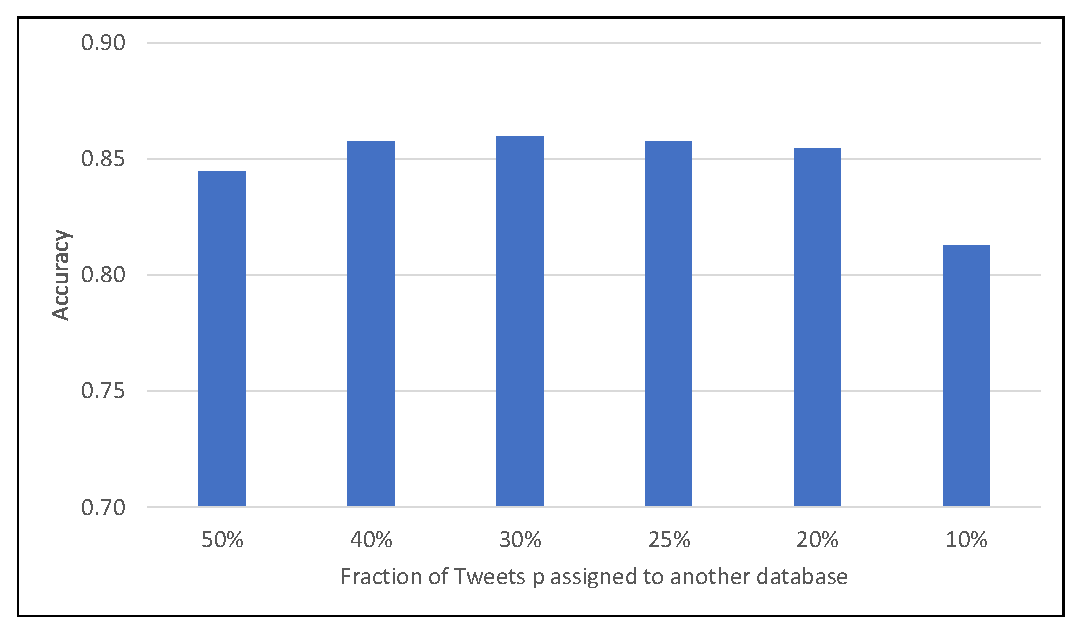
\includegraphics[width = 0.8\textwidth]{figures/sample_accuracy}
    \subcaption{User Linkage results for different fractions of user belonging to each database.}
    \label{fig:split_test}
  \end{subfigure}

  \begin{subfigure}[b]{\textwidth}
		\centering
    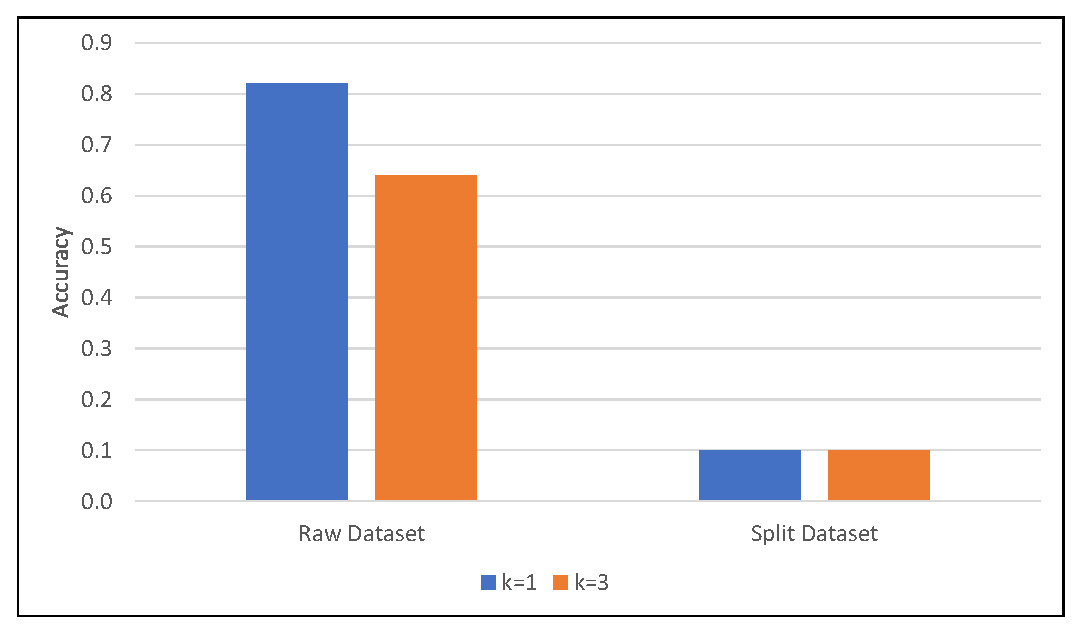
\includegraphics[width = 0.8\textwidth]{figures/split_accuracy}
    \subcaption{User Linkage results for linking Twitter and Instagram.}
    \label{fig:instagram}
  \end{subfigure}
  \caption{Classification Accuracy for different Social Networks.}
  \label{fig:split-results-ext}
	\figSpace
\end{figure}

{\bf Synthetic Database Split:} For the synthetic database, a fraction of $p$ Tweets is uniformly sampled from the Twitter dataset $\DB$, and pretend that this set belongs to a different social network $\DB^\prime$. In this sampled database $\DB^\prime$, the user-labels as ground-truth, which the algorithm tries to predict given the data in $\DB$ can be used. For this experiment, only trajectories having at least 10 tweets to sample from are considered. If uniform sampling of a trajectory yields an empty set, it is re-sampled.

{\bf Instagram Data:} Out of the 2.7 million tweets in the dataset, a significant portion of 204 thousand tweets is labelled as coming from the Instagram network. These Tweets were cross posted by the user, on both Instagram and Twitter. Thus, the Instagram database $\DB^I$ consists of all these cross-linked posts. For the Twitter database, two cases are evaluated. In the first case, the full dataset $\DB$ can simply be used, thus assuming that the Instagram observations were made in both datasets. In the second case, the database $\DB_T=\DB\setminus \DB_I$ is used, thus assuming that the Instagram observations were made in the Instagram network only.

The results on the synthetic database split are shown in Figure \ref{fig:split_test}.
For each value of $p$, 10 random samples of the database $\DB$ are obtained, and averaged the results in order to avoid effects generated due to random sampled. In all ten runs, the depicted values showed almost no deviation, all being in a $\pm 0.5\%$ interval. An even 50/50 split yields a correct linkage rate of almost $85\%$. Yet, this split becomes biased towards a smaller value $p$. This can be explained by having a larger sample in the training database $\DB$, on which the trajectories of $\DB^\prime$ are queried on. However, for $p=0.1$, this accuracy drops significantly. This can be explained by the previous experiments, showing that a sample of as little as three observations suffices for a high classification accuracy. However, since many of the trajectories only have $10-20$ observations, there is a high chance that a $10\%$ random sample may only have one or two observations.

For the Instagram-Twitter matching, the results are shown in Figure \ref{fig:instagram}, for the two cases of using the data as is, thus having all Instagram observations also present in the Twitter database, and the case of splitting the dataset, thus removing the Instagram observations from the Twitter trajectories. Using the raw dataset a prediction accuracy of roughly $80\%$ using $k=1$ nearest neighbor classification to build the bi-partite graph is observed.

In contrast, the case of splitting Instagram off of Twitter, the accuracy drops to about $10\%$. These disappointing results can be explained by making the hypothesis that users use Instagram and Twitter in different ways, such as using Instagram when on a far-away vacation, while also using Twitter in locations where you don't usually take a picture, such as work and home. Also, some of the users had all their tweets linked to Instagram, such that the algorithm had no training data left in the Twitter database, thus having to random guess the user. Thus, it appears that Twitter and Instagram are used differently by users, making the Instagram sample much harder to match than a uniform random sample taken from Twitter.
